\documentclass[a4paper,twoside,11pt]{book}
\usepackage[utf8]{inputenc}
\usepackage[T1]{fontenc}
\usepackage[english,german]{babel}
	
%%%%%%%%%%%%%%%%%%%%%%%%%%%% NAME AND TITLE %%%%%%%%%%%%%%%%%%%%%%%%%%%%%%%%%%%%%%%%%%%%
%% Bitte füllen Sie dieses mit ihren Daten aus.
\title{Schriftliche Ausarbeitung für Seminar Aspekte Verteilte Systeme}
\author{Zhang, Zijian}
\newcommand{\betreuer}{Dipl.-Inform. H. Tobaben}
\date{\today}
\newcommand{\art}{Seminarausarbeitung}  % Bachelorarbeit / Diplomarbeit / Studienarbeit
\newcommand{\studiengang}{Informatik (M.Sc.)}
\newcommand{\keywords}{HPC, Energiebedarf, Seminarausarbeitung}
%%%%%%%%%%%%%%%%%%%%%%%%%%%%%%%%%%%%%%%%%%%%%%%%%%%%%%%%%%%%%%%%%%%%%%%%%%%%%%%%%%%%%%%%

% Trennungsregeln
\usepackage{hyphenat}
\hyphenation{Grid--Informations-systeme Sche-du-ler Sche-du-ling Per-for-mance Meta-sche-duler  Pla-gi-ats-prü-fung}

\usepackage{amssymb}							% provides mathmatical math symbols such as dots, arrows, etc.
\usepackage{amsmath}							% provides align environment
\usepackage{listings}
\lstset{captionpos=b,frame=single}
\usepackage[german]{fancyref}
%% for fancy refereing to listings.
\newcommand*{\fancyreflstlabelprefix}{lst}

\fancyrefaddcaptions{english}{%
  \providecommand*{\freflstname}{listing}%
  \providecommand*{\Freflstname}{Listing}%
}

\fancyrefaddcaptions{german}{%
  \providecommand*{\freflstname}{listing}%
  \providecommand*{\Freflstname}{Listing}%
}

\frefformat{plain}{\fancyreflstlabelprefix}{\freflstname\fancyrefdefaultspacing#1}
\Frefformat{plain}{\fancyreflstlabelprefix}{\Freflstname\fancyrefdefaultspacing#1}

\frefformat{vario}{\fancyreflstlabelprefix}{%
  \freflstname\fancyrefdefaultspacing#1#3%
}
\Frefformat{vario}{\fancyreflstlabelprefix}{%
  \Freflstname\fancyrefdefaultspacing#1#3%
}

%% 1.5 facher Zeilenabstand.
\usepackage[onehalfspacing]{setspace}

\makeatletter
\let\thetitle\@title
\let\theauthor\@author
\let\theday\@date
\makeatother

\usepackage{geometry}
\geometry{a4paper,left=35mm,right=25mm, top=2.5cm, bottom=2.5cm}

% Metadaten
\usepackage[
	colorlinks=true,
	linkcolor=black,						% enable for printing!
	urlcolor=black,						  % enable for printing!
	citecolor=black,						% enable for printing!
	%pdfstartview=Fit,						% fits the page to the window; other options: FitH/FitV (horiz./vert.)...
	%pdfpagelayout=TwoPageLeft,		% the way pages are displayed, options: SinglePage, OneColumn, TwoColumnLeft|Right, TwoPageLeft|Right
	final=true,									% turn on all processing options
	plainpages=false,						% Forces page anchors to be named by the arabic form of the page number, rather than the formatted form.
	pdfpagelabels]							% set PDF page labels
	{hyperref}
\hypersetup{
  pdftitle={\thetitle},
  pdfauthor={\theauthor},
  pdfsubject={\keywords}
}

\usepackage[nopostdot,nonumberlist,acronym]{glossaries}
%\makeglossaries

\makenoidxglossaries
%%%%%%%%%%%%%%%%%%%%%%%%%%%%%%%%%%%%%%%%%%%%%%%%%%%%%%%%%%%%%
%%                                                         %%
%%            Fügen sie hier alle Abkürzungen ein,         %%
%%                 welche Sie benutzen                     %%
%%                                                         %%
%%%%%%%%%%%%%%%%%%%%%%%%%%%%%%%%%%%%%%%%%%%%%%%%%%%%%%%%%%%%%

%% Name für Befehl \gls{} / Abkürzung / Ausgeschrieben
\newacronym{dcsec}{DCSec}{Distributed Computing \& Security Research Group}
\newacronym{mpi}{MPI}{Message Passing Interface}
\newacronym{omp}{OpenMP}{Open Multi-Processing}
\newacronym{pag}{PAG}{Per Anhalter durch die Galaxis}
\newacronym{xml}{XML}{eXtendable Markup Language}

%% Mehr informationen können unter https://www.ctan.org/pkg/glossaries?lang=de gefunden werden.

\usepackage{graphicx}
% sorgt dafür, dass LaTeX in images nach den Bildern sucht und der Ordner "etwas" aufgeräumter ist.
\graphicspath{ {./images/} {./graphics/} }


\usepackage{fancyhdr}
\pagestyle{fancy}
\fancyhf{} % sets both header and footer to nothing
\renewcommand{\headrulewidth}{0pt}
\parindent 0pt

\usepackage{helvet}
\renewcommand{\familydefault}{\sfdefault}
\fontfamily{phv}\selectfont


%%%%%%%%%%%%%%%%%%%%%%%%%%%%%%%%%%%%%%%%%%%%%%%%%%%%%%%%%%%%%%%%%%%%%%%%%%%%%%%%%%%%%%%%
%% Falls Sie noch weitere Pakete benötigen können diese hier eingebunden werden.

%\usepackage{...}

%%%%%%%%%%%%%%%%%%%%%%%%%%%%%%%%%%%%%%%%%%%%%%%%%%%%%%%%%%%%%%%%%%%%%%%%%%%%%%%%%%%%%%%%

\setlength{\headheight}{13.6pt}
\begin{document}

\frontmatter
%%%%%%%%%%%%%%%%%%%%%%%%%%%%%%%%%%%%%%%%%%%%%%%%%%%%%%%%%%%%%
%%                                                         %%
%%    Hier sollten von ihrer Seite aus keine Änderungen    %%
%%                  notwendig sein.                        %%
%%                                                         %%
%%%%%%%%%%%%%%%%%%%%%%%%%%%%%%%%%%%%%%%%%%%%%%%%%%%%%%%%%%%%%

\newgeometry{left=3cm,right=4cm, top=3cm, bottom=3.5cm}
\begin{titlepage}

%
% Logos
%

\includegraphics[height=1cm]{logo_dcsec} \hfill

\includegraphics[height=1cm]{logo_luh}

\vspace{-3mm}

\rule{\textwidth}{1pt}

\vspace{5mm}

\large

Gottfried Wilhelm Leibniz Universität Hannover

Institut für Verteilte Systeme

Distributed Computing \& Security Group

\vspace{4.0cm}

\art\\
im Studiengang \studiengang

\vspace{1.0cm}
\huge{\thetitle}

\vfill


\large
\begin{tabular}{p{3cm}l}
Verfasser:    & \theauthor\\
Betreuer:     & \betreuer\\
Datum:        & \theday
\end{tabular}


\end{titlepage}

\fancyfoot[C]{\thepage}

\tableofcontents

%% sorgt dafür, dass Verzeichnisse nicht auf ungeraden Seiten erscheinen, sondern nacheinander.
\makeatletter
\@openrightfalse
\makeatother

% Hier kommt das Abbildungsverzeichnis.
\listoffigures

% Hier kommt eine Liste der Tabellen.
\listoftables

% Codeverzeichnis
\renewcommand*{\lstlistlistingname}{Codeverzeichniss}
\lstlistoflistings

\printnoidxglossaries

%\printglossary[title=Nomenclature]

\mainmatter
\renewcommand{\headrulewidth}{0.4pt}
\fancyhead[OR]{\fontfamily{phv}\selectfont \rightmark}
\fancyhead[EL]{\fontfamily{phv}\selectfont \leftmark}

\makeatletter
\@openrighttrue
\makeatother

%%%%%%%%%%%%%%%%%%%%%%%%%%%%%% HAUPTTEIL %%%%%%%%%%%%%%%%%%%%%%%%%%%%%%%%%
%% binden sie hier Ihre anderen LaTeX Dateien ein.
\chapter{HPC}
\label{chap:HPC}

\section{Was ist HPC}
\label{sec:Was ist HPC}
HPC(Auf Englisch High Performance Computing), oder Rechnen mit dem Hilfer von Superrechner, ist typischweise Supercomputer mit großen Anzahl der Prozessoren, die auf gemeisame Peripheriegeräte und eine teiweise gemeisamen Hauptspeicher zugreifen können, die die auf dem Wikipedia beschrieben werden. 

\section{Warum HPC}
\label{sec:Warum HPC}
Um die Lösung maßstabreicher Probleme zu finden. Diese Probleme hat dem Merkmal, dass sie auf viele homogenisierende Teilprobleme bestanden, zum Beispiel die auf dem Bereich Hydromechanik, Biologie oder atmosphärische Wissenschaften. Um das Rechnungsprozess zu beschleunigen, ist parallele Rechnung sehr hilfreich. Das ist auch der Grund dafür, warum Supercomputers werden von Institute alle Land immer noch untersucht.

\section{HPC und Energiebedarf}
\label{sec:HPC und Energiebedarf}
Unter der gleichem Architechtur besitzt ein Supercomputer je mehr Prozessoren verbraucht es mehr Energie. Mit der Leistung von 93.000,00 TeraFLOPS beträgt der Energiebedarf von Sunway TaihuLight 15.370kW, was ist eigentlich zehr energieaufwändig. Aber dieser Zustand ist verbesserbar. Eine Seit durch den Fortschritten der Technik kann man die Architektur von Supercomputer monifizieren, um zum schluß die Energiebedarf per Prozessor zu senken, andere Seit ist die Softwareimpimentation auch verbesserbar. In diser Ausarbeitung biete ich ein paar Vergleichen an, der viele Energiebedarf-relevante Aspekte identifizieren.

\chapter{Versuchen}
\label{chap:Versuchen}

\section{Untersuchungsplattform}
\label{sec:Untersuchungsplattform}
Unsere Untersuchung wurde durchgeführt auf dem Plattform wie unter:

\begin{table}[htbp]
\begin{center}
\begin{tabular}{ l | l }
	Hardwaresystem 	& ODROID-XU3 Lab Environment(mit ARM Cortex-A7\\
					& 1.4Ghz und Cortex-A15 2.0Ghz big.LITTLE\\
					& architecture jeweils 4 kerne)\\ \hline
	Betribssystem 	& Ubuntu 15.10 mit ssh Zugriff und shared\\
					& storage durch NFS server\\ \hline
	Test-Benchmark 	& NAS Parallel Benchmarks\\ \hline
	Tasks 			& LU Dekomposition und Gauß'sche Elimination(LU)\\ \hline
					& und konjugierender Gradient(CG)\\ \hline
	Task-Maßstab	& siehe Tablett \ref{tab:Task-Massstab}\\ \hline
	Implementationssprache 	& Java\\ \hline
	Implementationsmethode 	& OpenMP und MPI(Message Passing\\
							& Interface)\\ \hline
	Messungsgeräte & ODROID Smart Power Device 
\end{tabular}
\end{center}
\label{tab:Untersuchungsplattform}
\caption{Untersuchungsplattform}
\end{table}

\begin{table}[htbp]
\begin{center}
\begin{tabular}{l|l|l|l}
	&			&Class A 	&Class B\\ \hline
CG 	&Size		&14000		&75000\\
	&Iteration	&15			&75\\ \hline
LU 	&Size		&64x64x64	&102x102x102\\
	&Iteration	&250		&250\\
\end{tabular}
\end{center}
\label{tab:Task-Massstab}
\caption{Task-Maßstab}
\end{table}

\section{Energiebedarf-relevante Aspekte}
\label{sec:Energiebedarf-relevante Aspekte}
\subsection{Energiebedarf und Architektur}

\begin{figure}[ht]
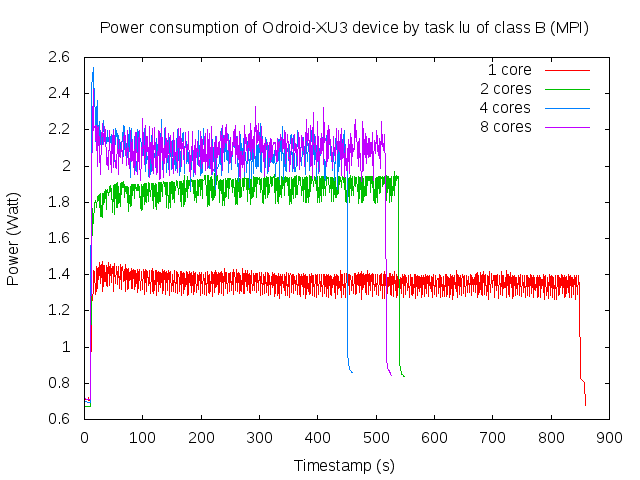
\includegraphics[width=\textwidth]{cores_power}
\caption[Leistung und Kernenutzung]{Leistung und Kernenutzung}
\label{fig:Leistung und Kernenutzung}
\end{figure}

\begin{figure}[ht]
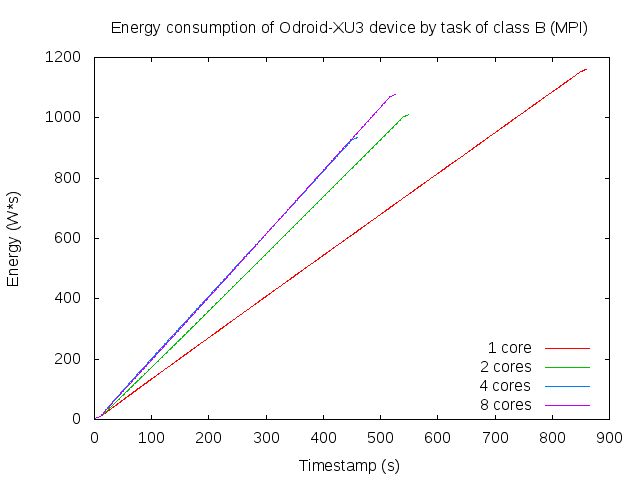
\includegraphics[width=\textwidth]{cores_energy}
\caption[Energiebedarf und Kernenutzung]{Energiebedarf und Kernenutzung}
\label{fig:Energiebedarf und Kernenutzung}
\end{figure}

\begin{figure}[ht]
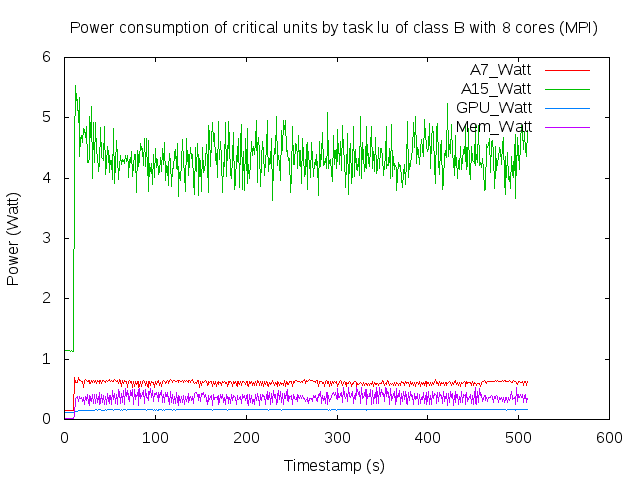
\includegraphics[width=\textwidth]{units_power}
\caption[Leistung kritischer Teilen]{Leistung kritischer Teilen}
\label{fig:Leistung kritischer Teilen}
\end{figure}

Wie gezeigt in Abbildung \ref{fig:Leistung und Kernenutzung} und sein Integral Abbildung \ref{fig:Energiebedarf und Kernenutzung}. Die Rechnung befasst sich um das Task von LU und mit BWenn es nur ein Kern aktiviert ist, ist die Energiebedarf des Computersystems am höchsten und dauert die Rechung am längsten. Deshalb die Konfiguration mit nur ein aktivierende Kern ist auf jeden Fall nicht effizient. 

Aber es ist auch komisch, dass die Zeit- und Energiebedarf des Task von 8 Kerne sind beide höher als die von 4 Kerne. Laut der Dokumentation von ODROID-XU3 kann man feststellen, dass es 4 Kerne von Cortex-A7 und 4 Kerne von Cortex-A15 auf der Tafel sich befindet. Wenn es nur 4 Kerne aktiviert ist, sind die 4 Kerne mit niedrigere ID, d.h. 4 Kerne von Cortex-A7 laufbar. 

Der Grunden dafür kann man mit dem Hilfe Dokumentationen und Versuchergebnisse vermuten. Rechnungsdatenumtauschung innerhalb ein CPU ist immer noch effizienter als die über 2 CPUs. Darum ist die Zeitbedarf mit 4 Kerne nideriger. Beschrieben von Webseite von ARM und in Beachtung von Messungsergebnis in Abbildung \ref{fig:Leistung kritischer Teilen}, ist die Leistung des Cortex-A15 höher als die des Cortex-A7 und für die Energiebedarf vice versa. Deshalb für eine Rechnungsarbeit mit so moderatem Maßtab soll man die energieeffiziente CPUs beforzugen.
\chapter{Codes}
\label{chap:Codes}

In disem Kapitel werden alle automatisierte Skripte (zu kompilieren und messen, beziehungsweise für die Abbildungsherstellung) dargestellt

\begin{lstlisting}[label=lst:compile.py, caption={compile.py}]
import os

result_dir = "~/res"
base_dir = "~/LAB/NAS/"
ver_dir= "NPB3.3.1/"
ver_short = "NPB3.3"
impls= ["MPI", "OMP"]

benchmark_names = ["CG", "LU"]
class_names = ["S", "W", "A", "B", "C", "D"]

for impl in impls:
     cp_command = "cp "+base_dir+impl+"/make.def "+
     			  base_dir+ver_dir+ver_short+
     			  	"-"+impl+"/config/"

     os.system(cp_command)

     for bn in benchmark_names:
         for cn in class_names:
             for core_num in [1,2,4,8]:
                 make_command = "cd "+base_dir+ver_dir+
                                ver_short+"-"+impl+
                                "/;make "+bn

                 if impl == "MPI":
                     make_command+=" NPROCS="+
                                   str(core_num)

                 elif core_num>1:
                     break

                 make_command += " CLASS="+cn
                 os.system(make_command)
\end{lstlisting}

\begin{lstlisting}[label=lst:meassure.sh, caption={meassure.sh}]
#!/bin/bash

res_dir="/home/user5/res/"
if [ ! -f $resultdir ];
then
 mkdir -p $resultdir
fi

basedir="/home/user5/LAB/NAS/"
verdir="NPB3.3.1/"
vershort="NPB3.3"

impls="MPI OMP"
benchmark_names="cg lu"
class_names="A B"

core_nums="1 2 4 8"

mes_sensor="stdbuf -oL read-xu3-sensors -c -t"
mes_power="stdbuf -oL smartpower -c -t"

for impl in $impls;
do
 for bn in $benchmark_names;
 do
  for cn in $class_names;
  do
   for core_num in $core_nums;
   do
    res_folder=$res_dir"/"$impl"/"
    
    if [ ! -f $res_folder ];
    then
     mkdir -p $res_folder
    fi
    
    sensor_res_filename=$res_folder$bn"."\
                        $cn"."$core_num\
                        ".sensor.txt"
    power_res_filename=$res_folder$bn"."\
                       $cn"."$core_num\
                       ".power.txt"
    
    if [ -e $sensor_res_filename ] && 
       [ `wc -l $sensor_res_filename | 
         cut -f 1 --delimiter=" "` != "0" ] && 
       [ -e $power_res_filename ] &&
       [ `wc -l $power_res_filename | 
         cut -f 1 --delimiter=" "` != "0" ];
    then
     continue
    fi
    
    ($mes_sensor)>$sensor_res_filename& 
    pid_mes_sensor=$!
    ($mes_power)>$power_res_filename&
    pid_mes_power=$!

    sleep 10 
    
    cd "/home/user5/LAB/NAS/NPB3.3.1/NPB3.3-"$impl"/bin"
    if [ $impl == "MPI" ];
    then
     run_cmd="mpirun.mpich -np $core_num ./"\
             $bn"."$cn"."$core_num
    else
     export OMP_NUM_THREADS=$core_num
     run_cmd="./"$bn"."$cn".x"
    fi
    
    ($run_cmd)
    sleep 10
    
    kill $pid_mes_sensor
    kill $pid_mes_power
    
    sync
    sleep 2
   done
  done
done
done
\end{lstlisting}

\begin{lstlisting}[label=lst:draw.p, caption={draw.p}]
set term png
unset log
unset label
set xtic auto
set ytic auto
set datafile separator ","
set key right top

set title "Power consumption of Odroid-XU3 device by\
          task lu of class B (MPI)"
set xlabel "Timestamp (s)"
set ylabel "Power (Watt)"
set output "cores_power.png"
plot\
    "MPI/lu.B.1.power.txt" u 0:3 t "1 core" with line,\
    "MPI/lu.B.2.power.txt" u 0:3 t "2 cores" with line,\
    "MPI/lu.B.4.power.txt" u 0:3 t "4 cores" with line,\
    "MPI/lu.B.8.power.txt" u 0:3 t "8 cores" with line;


set title "Power consumption of critical units by task\
          lu of class B with 8 cores (MPI)"
set output "units_power.png"
plot\
    "MPI/lu.B.8.sensor.txt" u 0:4 t "A7_Watt" with line,\
    "MPI/lu.B.8.sensor.txt" u 0:7 t "A15_Watt" with line,\
    "MPI/lu.B.8.sensor.txt" u 0:10 t "GPU_Watt" with line,\
    "MPI/lu.B.8.sensor.txt" u 0:13 t "Mem_Watt" with line


set title "Power consumption of Odroid-XU3 device by\
          different tasks (MPI)"
set output "tasks_power.png"
plot\
    "MPI/lu.B.8.power.txt" u 0:3 t "lu_8_cores" with line,\
    "MPI/lu.B.4.power.txt" u 0:3 t "lu_4_cores" with line,\
    "MPI/cg.B.8.power.txt" u 0:3 t "cg_8_cores" with line,\
    "MPI/cg.B.4.power.txt" u 0:3 t "cg_4_cores" with line;


set title "Power consumption of Odroid-XU3 device by\
          task lu of different scales (MPI)"
set output "scales_power.png"
plot\
    "MPI/lu.B.8.power.txt" u 0:3 t "B_8_cores" with line,\
    "MPI/lu.B.4.power.txt" u 0:3 t "B_4_cores" with line,\
    "MPI/lu.A.8.power.txt" u 0:3 t "A_8_cores" with line,\
    "MPI/lu.A.4.power.txt" u 0:3 t "A_4_cores" with line;
    

set title "Power consumption of Odroid-XU3 device by\
          task lu of class B with different implementations"
set output "implementations_power.png"
plot\
    "MPI/lu.B.8.power.txt" u 0:3 t "MPI_8_cores" with line,\
    "MPI/lu.B.4.power.txt" u 0:3 t "MPI_4_cores" with line,\
    "OMP/lu.B.8.power.txt" u 0:3 t "OpenMP_8_cores"\
     with line,\
    "OMP/lu.B.4.power.txt" u 0:3 t "OpenMP_4_cores"\
     with line;



set key right bottom
set xlabel "Timestamp (s)"
set ylabel "Energy (W*s)"
set title "Energy consumption of Odroid-XU3 device by task\
          of class B (MPI)"
sum1=0; sum2=0; sum4=0;sum8=0;
set output "cores_energy.png"
plot\
    "MPI/lu.B.1.power.txt" u 0:(sum1=sum1+$3) t "1 core"\
     with line,\
    "MPI/lu.B.2.power.txt" u 0:(sum2=sum2+$3) t "2 cores"\
     with line,\
    "MPI/lu.B.4.power.txt" u 0:(sum4=sum4+$3) t "4 cores"\
     with line,\
    "MPI/lu.B.8.power.txt" u 0:(sum8=sum8+$3) t "8 cores"\
     with line;


set title "Energy consumption of Odroid-XU3 device by\
          different tasks (MPI)"
sum1=0; sum2=0; sum4=0;sum8=0;
set output "tasks_energy.png"
plot\
    "MPI/lu.B.8.power.txt" u 0:(sum2=sum2+$3)\
     t "lu_8_cores",\
    "MPI/lu.B.4.power.txt" u 0:(sum1=sum1+$3)\
     t "lu_4_cores",\
    "MPI/cg.B.8.power.txt" u 0:(sum8=sum8+$3)\
     t "cg_8_cores",\
    "MPI/cg.B.4.power.txt" u 0:(sum4=sum4+$3)\
     t "cg_4_cores";


set title "Energy consumption of Odroid-XU3 device by\
          task lu of different scales (MPI)"
sum1=0; sum2=0; sum4=0;sum8=0;
set output "scales_energy.png"
plot\
    "MPI/lu.B.8.power.txt" u 0:(sum8=sum8+$3) t "B_8_cores",\
    "MPI/lu.B.4.power.txt" u 0:(sum4=sum4+$3) t "B_4_cores",\
    "MPI/lu.A.8.power.txt" u 0:(sum2=sum2+$3) t "A_8_cores",\
    "MPI/lu.A.4.power.txt" u 0:(sum1=sum1+$3) t "A_4_cores";
    

set title "Energy consumption of Odroid-XU3 device by\
          task lu of class B with different implementations"
sum1=0; sum2=0; sum4=0;sum8=0;
set output "implementations_energy.png"
plot\
    "MPI/lu.B.8.power.txt" u 0:(sum8=sum8+$3)\
     t "MPI_8_cores",\
    "MPI/lu.B.4.power.txt" u 0:(sum4=sum4+$3)\
     t "MPI_4_cores",\
    "OMP/lu.B.8.power.txt" u 0:(sum2=sum2+$3)\
     t "OpenMP_8_cores",\
    "OMP/lu.B.4.power.txt" u 0:(sum1=sum1+$3)\
     t "OpenMP_4_cores";


set title "Processing units' temperature monitoring on\
          running lu class B with 8 cores (MPI)"
set xlabel "Timestamp (s)"
set ylabel "Temperature (Celsius Degree)"
set output "mpi_temp.png"
plot\
    "MPI/lu.B.8.sensor.txt" u 0:23 t "CPU4_Temp" with line,\
    "MPI/lu.B.8.sensor.txt" u 0:24 t "CPU5_Temp" with line,\
    "MPI/lu.B.8.sensor.txt" u 0:25 t "CPU6_Temp" with line,\
    "MPI/lu.B.8.sensor.txt" u 0:26 t "CPU7_Temp" with line,\
    "MPI/lu.B.8.sensor.txt" u 0:26 t "GPU_Temp" with line;


set title "Processing units' temperature monitoring on\
          running lu class B with 8 cores (OpenMP)"
set output "openmp_temp.png"
plot\
    "OMP/lu.B.8.sensor.txt" u 0:23 t "CPU4_Temp" with line,\
    "OMP/lu.B.8.sensor.txt" u 0:24 t "CPU5_Temp" with line,\
    "OMP/lu.B.8.sensor.txt" u 0:25 t "CPU6_Temp" with line,\
    "OMP/lu.B.8.sensor.txt" u 0:26 t "CPU7_Temp" with line,\
    "OMP/lu.B.8.sensor.txt" u 0:26 t "GPU_Temp" with line;
\end{lstlisting}


%%%%%%%%%%%%%%%%%%%%%%%%%%%%%%%%%%%%%%%%%%%%%%%%%%%%%%%%%%%%%%%%%%%%%%%%%%


\appendix


%%%%%%%%%%%%%%%%%%%%%%%%%%%%%%% ANHÄNGE %%%%%%%%%%%%%%%%%%%%%%%%%%%%%%%%%%
%% binden sie hier Ihre LaTeX Dateien ein, welche zum Anhang gehören.

%%%%%%%%%%%%%%%%%%%%%%%%%%%%%%%%%%%%%%%%%%%%%%%%%%%%%%%%%%%%%%%%%%%%%%%%%%

\bibliographystyle{plain}
\bibliography{referenzen}

\end{document}
